\documentclass{beamer}
%\documentclass[handout]{beamer}

\mode<presentation>
{% AnnArbor
%\usetheme{AnnArbor}
  %\usetheme{Boadilla}
  \usetheme{CambridgeUS}
 %\usetheme{Madrid}
  \setbeamercovered{transparent}
}

\usepackage{fontspec,xltxtra,xunicode,moreverb}

\usepackage[french]{babel}
% \usepackage{beamerthemesplit} // Activate for custom appearance

\usepackage{listings}
\usepackage{color}

\definecolor{mygreen}{rgb}{0,0.6,0}
\definecolor{mygray}{rgb}{0.5,0.5,0.5}
\definecolor{mymauve}{rgb}{0.58,0,0.82}

\lstset{ 
  backgroundcolor=\color{white},   % choose the background color; you must add \usepackage{color} or \usepackage{xcolor}; should come as last argument
  basicstyle=\footnotesize,        % the size of the fonts that are used for the code
  breakatwhitespace=false,         % sets if automatic breaks should only happen at whitespace
  breaklines=true,                 % sets automatic line breaking
  captionpos=b,                    % sets the caption-position to bottom
  commentstyle=\color{mygreen},    % comment style
  deletekeywords={...},            % if you want to delete keywords from the given language
  escapeinside={\%*}{*)},          % if you want to add LaTeX within your code
  extendedchars=true,              % lets you use non-ASCII characters; for 8-bits encodings only, does not work with UTF-8
  firstnumber=1000,                % start line enumeration with line 1000
  frame=single,	                   % adds a frame around the code
  keepspaces=true,                 % keeps spaces in text, useful for keeping indentation of code (possibly needs columns=flexible)
  keywordstyle=\color{blue},       % keyword style
  language=Python,                 % the language of the code
  morekeywords={*,...},            % if you want to add more keywords to the set
  numbers=left,                    % where to put the line-numbers; possible values are (none, left, right)
  numbersep=5pt,                   % how far the line-numbers are from the code
  numberstyle=\tiny\color{mygray}, % the style that is used for the line-numbers
  rulecolor=\color{black},         % if not set, the frame-color may be changed on line-breaks within not-black text (e.g. comments (green here))
  showspaces=false,                % show spaces everywhere adding particular underscores; it overrides 'showstringspaces'
  showstringspaces=false,          % underline spaces within strings only
  showtabs=false,                  % show tabs within strings adding particular underscores
  stepnumber=1,                    % the step between two line-numbers. If it's 1, each line will be numbered
  stringstyle=\color{mymauve},     % string literal style
  tabsize=2,	                   % sets default tabsize to 2 spaces
  % title=\lstname                   % show the filename of files included with \lstinputlisting; also try caption instead of title
}


%% No navigation symbol.
\setbeamertemplate{navigation symbols}{}
\beamertemplatenavigationsymbolsempty

%\setbeameroption{hide notes}

% \newcommand{\mypause}{\pause}
\newcommand{\mypause}{~}

\newcommand{\mypauseBeforeExercise}{\pause}

\newcommand{\elvrm}{\rm}
\newcommand{\fivrm}{\rm}
\newcommand{\sixrm}{\rm}
\newcommand{\sevrm}{\rm}
\newcommand{\egtrm}{\rm}
\newcommand{\ninrm}{\rm}
\newcommand{\tenrm}{\rm}
\newcommand{\twlrm}{\rm}
\newcommand{\frtnrm}{\rm}
\newcommand{\svtnrm}{\rm}
\newcommand{\twtyrm}{\rm}
\newcommand{\twfvrm}{\rm}

\newcommand{\ex}{{\bf Exemple}}
\newcommand{\afor}{\bf for}
\newcommand{\ato}{\bf to}
\newcommand{\ado}{\bf do}
\newcommand{\aendo}{\bf endo}
\newcommand{\esp}{\hspace{0.5cm}}

\newcommand{\sal}{\sum_i \mu_i}
\newcommand{\sbet}{\sum_j \nu_j}
\newcommand{\If}{\mbox{\bf if }}
\newcommand{\Then}{\,\mbox{\bf then }}
\newcommand{\titre}[1]{\title{{{\color{red} \large \bf #1}}}}

% Needed for course 2.
\newcommand{\Zn}{{\bf Z}^n}
\newcommand{\Z}{{\bf Z}}
\newcommand{\N}{{\bf N}}
\newcommand{\Np}{{\bf N}^p}

\newcommand{\alfa}{\textsc{alpha}}
\newcommand{\alfacase}{\mbox{\bf case}}
\newcommand{\alfaesac}{\mbox{\bf esac}}
\newcommand{\zset}{\mathbb{Z}}

\newcommand{\sys}{{\bf system}}
\newcommand{\real}{{\bf real}}
\newcommand{\of}{{\bf of}}
\newcommand{\lett}{{\bf let}}
\newcommand{\tel}{{\bf tel}}
\newcommand{\returns}{{\bf returns}}
\newcommand{\boolean}{{\bf boolean}}
\newcommand{\true}{{\bf true}}
\newcommand{\false}{{\bf false}}

\newcommand{\pomme}{\texttt{cmd}}
\newcommand{\alalign}{{$\hookleftarrow$}}

\newcommand{\pyth}{{\sc Python}}
\newcommand{\prog}[1]{\alert{\texttt{#1}}}

\title{Introduction à l'informatique, avec \pyth{}}
% \author{Patrice Quinton}
\author{Lilian Besson}
\date{2020--2021\\Version du \today}

\institute% (optional, but mostly needed)
{
  %\inst{1}%
  ENS Rennes
  }

\date%[\today] % (optional, should be abbreviation of conference name)
[Info -- DEM -- 2020]{Initiation à l'informatique -- DEM -- 2020\\Module 5 (fin du cours)}
\logo{
\includegraphics[height=0.5cm]{logoENS.pdf}}

% Delete this, if you do not want the table of contents to pop up at
% the beginning of each subsection:
\AtBeginSection[]
{
  \begin{frame}<beamer>
    \frametitle{Plan du cours}
%    \tableofcontents[currentsection,currentsubsection]
\tableofcontents[currentsection,currentsubsection,hideallsubsections]
  \end{frame}
}

\begin{document}

\frame{\titlepage}

\section[Outline]{}
\frame{\tableofcontents}
\frame
{
\frametitle{``Résumé des épisodes précédents''}
{
On a vu:
\begin{itemize}
  \item comment accéder à l'ordinateur via son \prog{terminal}
  \item quelques commandes simples permettant de se déplacer dans la \prog{hiérarchie des fichiers}
  \item comment démarrer \pyth{}
  \item comment écrire un programme avec l'éditeur \prog{idle}
  \item les \prog{variables}, leur \prog{type} (\prog{int}, \prog{float}, \prog{bool}, \prog{str}), l'affectation,
  \item les \prog{conditions} et instructions conditionnelles
  \item la boucle \prog{while},
  \item les chaînes de caractères (\prog{str} et les )\prog{listes},
  \item les fonctions.
\end{itemize}
}
}

\section{TP pendant une heure : algorithmes numériques}

\frame
{
\frametitle{Activité à faire pendant une heure}

J'aimerai vous faire programmer une fonction qui implémente un algorithme de calcul approchée de $\sqrt{x}$, selon la méthode dite des Babyloniens (cf CM1).

{\footnotesize
\begin{block}{A faire}
\begin{itemize}
\item Par binômes, suivez les instructions données dans le document,
\item Appelez moi si vous avez besoin d'aide,
\item Jouez avec les paramètres de votre algorithme et comparez la qualité et la précision des résultats obtenus : nombre maximum d'itération, précision, ...
\item Quand vous aurez fini pour $\sqrt{x}$, essayez de faire pareil pour $\exp(x)$ et $\cos(x)$ ou $\sin(x)$ (les instructions sont dans la suite du document).
\end{itemize}
\end{block}
}
}


% \section{L'algorithme de la crêpière}

% \frame
% {
% \frametitle{Ranger un tas de crêpes}
% On est maintenant en mesure de ranger un tas de crêpes... ou presque.
% {\footnotesize
% \begin{block}{Coder un tas de crêpes}
% \begin{itemize}
% \item On représente un tas de crêpes par une \alert{liste} de cinq entiers, qui indiquent leur
% taille\mypause{}
% %\item Pour l'instant, on ne va pas s'occuper de savoir si la crêpe est à l'endroit ou pas\mypause{}
% \item Par exemple: \prog{tas = [2,1,4,5,3]} représente un tas de crêpes (celle du bas en
% premier)\mypause{}
% \item On pourrait prendre d'autres représentations...
% \end{itemize}
% \end{block}
% }
% }

% \frame
% {
% \frametitle{Diviser pour mieux régner}
% Un peu de réflexion
% {\footnotesize
% \begin{block}{Décomposer en opérations plus simples}\mypause{}
% \begin{itemize}
% \item Partons de \alert{\texttt{[2,1,4,5,3]}}. On a dit qu'il nous faut trouver la plus
% grande crêpe (ici, c'est la 4ème), puis retourner le tas du haut, à partir de
% cette crêpe. Si on fait cela, on doit arriver au nouveau tas \texttt{[2,1,4,\alert{3,5}]}.\mypause{}
% \item Puis, on a dit qu'on retourne tout le tas, on doit donc ensuite arriver
% au tas codé \alert{\texttt{[5,3,4,1,2]}}\mypause{}
% \item Il nous faut donc savoir faire plusieurs choses: \mypause{}
% \begin{enumerate}
% \item trouver le rang du plus grand élément de la liste, \mypause{}
% \item retourner le haut de la pile, à partir du plus grand élément \mypause{}
% \item retourner tout un tas. \mypause{}
% \end{enumerate}
% \end{itemize}
% \end{block}
% }
% }

% \section{La fonction \prog{rangMax}}

% \frame
% {
% \frametitle{Résoudre chacun des problèmes: \prog{rangMax}}
% \begin{itemize}
% \item On programme une fonction \prog{rangMax} qui appliquée
% à une liste de 5 entiers, rend le numéro de son plus grand élément.\mypause{}
%     \begin{itemize}
%         \item \alert{\texttt{rangMax( [1,3,5,4,2] )}} me donne \alert{\texttt{2}}
%         \item \alert{\texttt{rangMax( [] )}} me donne \alert{\texttt{-1}} par convention
%     \end{itemize}\mypause{}
% \item Pour rappel, voici le programme que nous avions écrit:
% \alert{{\footnotesize
% \verbatiminput{../Programmes-Python/rangMax.py}
% }}
% \end{itemize}
% }


% \frame
% {
% \frametitle{En pratique}
% \begin{itemize}
% \item Dans \textsc{Kit-3}, vous trouverez un \alert{squelette} de programme
% appelé \textsc{crépier-1.py}\mypause{}
% \item Recopiez-le dans un de vos répertoires\mypause{}
% \item Modifiez-le pour réaliser la fonction \prog{rangMax} et pour {\em tester}
% cette fonction\mypause{}
% \end{itemize}
% (Solution crépier-2.py)
% }

% \frame{
% \frametitle{Voici le squelette}
% {\footnotesize
% \alert{
% \verbatiminput{../Programmes-Python/crépier-1.py}
% }}
% }

% \section{Fonction \prog{retournerTas}}

% \frame
% {
% \frametitle{Second problème à résoudre: \prog{retournerTas}}
% \begin{itemize}
% \item On crée une fonction \alert{\texttt{retournerTas( tas, numéro )}} qui
% rend \alert{\texttt{tas}} où la pile qui commence à l'indice \texttt{numéro}
% est retournée. \mypause{}
% \begin{itemize}
% \item \alert{\texttt{retournerTas( [1,3,5,4,2], 2 )}} donne \alert{\texttt{[1,3,2,4,5]}}
% \item \alert{\texttt{retournerTas( [1,2,3,4,5], 0 )}} donne \alert{\texttt{[5,4,3,2,1]}}
% \end{itemize}
% \item Rappel:
% \begin{itemize}
% \item \alert{tas.reverse()} permet d'inverser la liste tas.
% \item \alert{x = tas[i:j]} met dans la variable \alert{x} la sous-liste
% de \alert{tas} entre les éléments i et j-1.
% \item \alert{liste1 + liste2} permet la {\em concaténation} des listes
% \alert{liste1} et \alert{liste2}
% \end{itemize}
% \item À faire: recopier le programme contenant la fonction \alert{rangMax},
% puis modifiez-le pour ajouter la nouvelle fonction
% \end{itemize}
% (Solution: crépier-3.py)
% }

% \frame{
% \frametitle{Et maintenant?}
% {\footnotesize
% \begin{block}{Ce dont on dispose}
% \begin{itemize}
% \item On a une fonction qui permet de trouver le rang (numéro) de la plus grande
% crèpe
% \item On a une autre fonction qui permet de retourner une pile de crêpes à partir
% d'un numéro donné
% \end{itemize}
% \end{block}
% \begin{block}{Ce qu'il faut faire}
% On part de \prog{tas = [2,1,5,3,4]}
% \begin{itemize}
% \item \prog{r = rangMax(tas)} donne \prog{2}
% \item \prog{tas = retournerPile(tas,r)} donne \prog{[2,1,4,3,5]}
% \item \prog{tas = retournerPile(tas,0)} donne \prog{[5,3,4,1,2]}
% \item et ensuite?
% \end{itemize}
% \end{block}
% }
% }

% \section{Le programme complet}

% \frame{
% \frametitle{Esquisse du programme}
% \begin{block}{Ce qu'il faut faire}
% {\footnotesize
% Dans la partie \prog{main} (programme principal) de votre programme,
% ajouter les instructions
% qui permettent d'effectuer le
% rangement d'un tas de crêpes, en poursuivant ce que nous venons
% d'esquisser
% }
% \end{block}
% (Solution: crépier-4.py)
% }

% \frame{
% \frametitle{Le programme complet}
% \begin{block}{Ce qu'il faut faire}
% {\footnotesize
% Remplacez ce programme par une boucle \prog{while}, ce qui permet
% de ranger des tas de crêpes de taille quelconque\mypause{}
% }
% \end{block}
% (Solution: crépier-5.py)
% }

% \frame{
% \frametitle{Sous forme d'une fonction}
% \begin{block}{Ce qu'il faut faire}
% {\footnotesize
% Remplacez ce programme par une fonction \alert{rangerCrèpes},
% ce qui permet d'appeler le programme sur une liste quelconque de
% crèpes
% }
% \end{block}
% (Solution: crépier-6.py)
% }

% \frame{
% \frametitle{Une version sans boucle While}
% \begin{block}{Un programme récursif}
% {\footnotesize
% On peut, dans certains langages, rappeler une fonction
% \alert{{\em à l'intérieur d'elle-même}}.
% }
% \end{block}
% (Solution: crépier-7.py)
% }

\section{Auto évaluation}

\frame{
\frametitle{Auto évaluation}
\begin{itemize}
\item Je vous ai distribué un formulaire d'auto évaluation,
\item Remplissez le honnêtement, du début à la fin,
\item Ce n'est pas noté, c'est pour que \textbf{vous} évaluiez votre compréhension du cours.
\end{itemize}
}


\section{Petite histoire : Katie Bouman}

\frame
{
\frametitle{Katie Bouman : un exemple de \textit{success story} entre \textit{data science} et astronomie}
% {\footnotesize
\begin{itemize}
\item Née aux USA en XXX.
\item TODO
\item TODO
\item TODO
\item TODO
\end{itemize}
% }
}

\frame
{
\frametitle{Katie Bouman}
{\footnotesize
% \vspace*{5pt}
\begin{figure}
  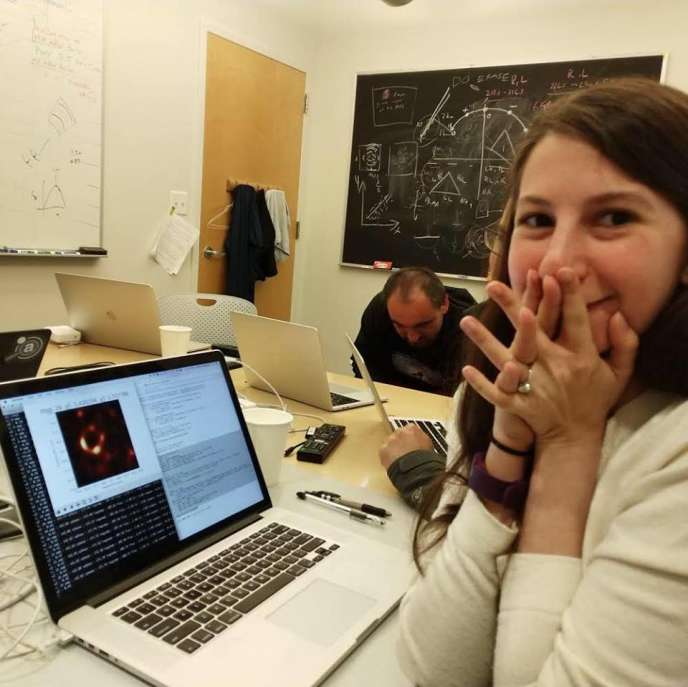
\includegraphics[height=150pt]{katie_bouman.jpg}
\end{figure}
\begin{itemize}
  \item Énorme volume utilisé pour stocker les données !
  \item A mettre en parallèle avec la précédente ``petite histoire'' parlant de Margaret Hamilton.
  % https://www.lemonde.fr/sciences/article/2019/04/12/katie-bouman-la-traqueuse-de-trou-noir-propulsee-malgre-elle-superstar-des-femmes-de-science_5449542_1650684.html
\end{itemize}
}
}


\section{Conclusion}

\frame{
\frametitle{En résumé}
\begin{itemize}
\item On a vu \alert{comment préparer un programme \pyth{}}
\item Comment en \alert{vérifier la syntaxe} (\texttt{check})
\item Comment le \alert{sauvegarder}
\item Comment lancer son \alert{exécution}
\item Comment utiliser des \alert{entiers}, des \alert{flottants}, des \alert{chaînes} de caractères, des \alert{listes},
\item Comment définir et utiliser des \alert{fonctions}
\end{itemize}
}

\frame{
\frametitle{Devoir maison à faire pour conclure le cours}
Si vous voulez travailler encore un peu le cours, essayez de programmer l'``algorithme de la crêpière'' vu au premier cours CM1.

Une solution commentée est disponible sur le site du cours.
\url{https://perso.crans.org/besson/teach/intro_num_DEM_2020/2020-DEM/}
}

\frame{
\frametitle{Conclusion : ``take home message'' du cours}
Si vous voulez travailler encore un peu le cours, essayez de programmer l'``algorithme de la crêpière'' vu au premier cours CM1.

Une solution commentée est disponible sur le site du cours.
\url{https://perso.crans.org/besson/teach/intro_num_DEM_2020/2020-DEM/}
}

\end{document}

